\documentclass[aspectratio=169]{beamer}
\usepackage{animate}
\usepackage{xcolor}
\usepackage[absolute,overlay]{textpos}
\usepackage[textfont={scriptsize}]{caption}
\usepackage{booktabs}
\usepackage{bm}
\usepackage[normalem]{ulem}
\usepackage{subcaption}
\usepackage{algorithm}
\usepackage{algorithmic}
\usepackage{setspace}

\usepackage{transparent}
\usetheme{Boadilla}

\newcommand\email[1]{\def\insertemail{#1}}
\newcommand{\placebottom}{\vskip0pt plus 1filll}
\providecommand\insertemail{\texttt{alefilot@auth.gr}}
% No slide numbering

\setbeamertemplate{footline}
{
\leavevmode%
\hbox{%
\begin{beamercolorbox}[wd=.3\paperwidth,ht=2.25ex,dp=1ex,center]{author in head/foot}%
\usebeamerfont{author in head/foot}\insertshortauthor~~(\insertshortinstitute)
\end{beamercolorbox}%
\begin{beamercolorbox}[wd=.5\paperwidth,ht=2.25ex,dp=1ex,center]{title in head/foot}%
\usebeamerfont{title in head/foot}\insertshorttitle
\end{beamercolorbox}%
%\begin{beamercolorbox}[wd=.2\paperwidth,ht=2.25ex,dp=1ex,right]{date in head/foot}%
%\usebeamerfont{date in head/foot}\insertshortdate{}\hspace*{2em}
%%#turning the next line into a comment, erases the frame numbers
%%\insertframenumber{} / \inserttotalframenumber\hspace*{2ex}
%\end{beamercolorbox}}%
\begin{beamercolorbox}[wd=.2\paperwidth,ht=2.25ex,dp=1ex,center]{date in head/foot}%
\usebeamerfont{date in head/foot}\insertemail{}
%#turning the next line into a comment, erases the frame numbers
%\insertframenumber{} / \inserttotalframenumber\hspace*{2ex}
\end{beamercolorbox}}%
\vskip0pt%
}

%remove navigation symbols
\setbeamertemplate{navigation symbols}{}

\usepackage{tikz}
\usetikzlibrary{matrix,backgrounds}
\usetikzlibrary{arrows.meta,chains,decorations.pathreplacing}
\usetikzlibrary{intersections}
\usetikzlibrary{angles, quotes}
\newcommand{\tikzxmark}{%
\tikz[scale=0.23] {
    \draw[line width=0.7,line cap=round] (0,0) to [bend left=6] (1,1);
    \draw[line width=0.7,line cap=round] (0.2,0.95) to [bend right=3] (0.8,0.05);
}}
\newcommand{\tikzcmark}{%
\tikz[scale=0.23] {
    \draw[line width=0.7,line cap=round] (0.25,0) to [bend left=10] (1,1);
    \draw[line width=0.8,line cap=round] (0,0.35) to [bend right=1] (0.23,0);
}}

% Highlight algorithm parts with color
\usetikzlibrary{calc}
\usetikzlibrary{fit}
\newcommand*{\tikzmk}[1]{\tikz[remember picture,overlay,] \node (#1) {};\ignorespaces}
%define a boxing command, argument = colour of box
\newcommand{\boxit}[1]{\tikz[remember picture,overlay]{\node[yshift=3pt,fill=#1,opacity=.25,fit={($(A)+(-0.038\linewidth,.3\baselineskip)$)($(B)+(.9\linewidth,-.3\baselineskip)$)}] {};}\ignorespaces}

% BOXES
\usepackage{environ}
\usepackage[many]{tcolorbox}
\NewEnviron{gg_box}{%
  \vspace{0.5cm}
  \begin{tcolorbox}[colback=black!5, colframe=white!80!, breakable]
  %\begin{tcolorbox}[colback=white!10, colframe=black!30!, breakable]
    \BODY
  \end{tcolorbox}
}

\definecolor{sticky_note_yellow}{cmyk}{0.0, 0.0, 0.06, 0.0, 1.00}
\NewEnviron{sticky_note_box}{%
  \vspace{0.5cm}
  \begin{tcolorbox}[colback = sticky_note_yellow, colframe=sticky_note_yellow, breakable]
    \BODY
  \end{tcolorbox}
}

\NewEnviron{bw_box}{%
  \vspace{0.5cm}
  \begin{tcolorbox}[colback=white!10, colframe=black!80!, arc=0pt,outer arc=0pt, breakable]
    \BODY
  \end{tcolorbox}
}

\NewEnviron{gw_box}{%
  \vspace{0.5cm}
  \begin{tcolorbox}[colback=white!10, colframe=black!10!, breakable]
    \BODY
  \end{tcolorbox}
}

\NewEnviron{bg_box}{%
  \vspace{0.5cm}
  \begin{tcolorbox}[colback=black!10, colframe=black!80!, arc=0pt,outer arc=0pt, breakable]
    \BODY
  \end{tcolorbox}
}

\definecolor{alg1}{RGB}{251,180,174}
\definecolor{alg2}{RGB}{255,255,204}
\definecolor{alg3}{RGB}{179,205,227}

\definecolor{alg4}{RGB}{229,245,224}
\definecolor{alg5}{RGB}{161,217,155}
\definecolor{alg6}{RGB}{49,163,84}


\definecolor{my_red}{rgb}{0.894,0.102,0.110}
\definecolor{my_blue}{RGB}{71 71 186}

\definecolor{exp1_blue}{RGB}{33 74 135}
\definecolor{exp1_green}{RGB}{76 176 74}
\definecolor{exp1_red}{RGB}{255 0 0}



\title{CBGL: Fast Monte Carlo Passive Global Localisation \\ of 2D LIDAR Sensor}
%\subtitle{}
\author[Alexandros Filotheou]{\small Alexandros Filotheou}
\institute[AUTh GR]{Aristotelian University of Thessaloniki (AUTh), Greece}
\date{}

\titlegraphic{
  \includegraphics[width=1cm]{./figures/auth_logo}\hspace*{-11.75cm}\vspace{-2cm}~%
}

\newlength\imageheight
\newlength\imagewidth

\begin{document}

\input{slides/00/slide_00.tex}
\begin{frame}[noframenumbering]{Summary}

\begin{overlayarea}{\textwidth}{3cm}
\leavevmode
  Given
  \begin{itemize}
    \item a single 2D LIDAR measurement
    \item the map of the sensor's environment
  \end{itemize}

  CBGL $\Rightarrow$ global localisation $\sim 1.0$ sec $ / 100 \text{m}^2$

\end{overlayarea}
\end{frame}

\begin{frame}[noframenumbering]{Summary}

\begin{overlayarea}{\textwidth}{3cm}
  Given
  \begin{itemize}
    \item a single 2D LIDAR measurement
    \item the map of the sensor's environment
  \end{itemize}

  CBGL $\Rightarrow$ global localisation $\sim 1.0$ sec $ / 100 \text{m}^2$, robust to

  \begin{itemize}
    \item varying maximum sensor range
    \item varying field of view
    \item sensor \& map noise
    \item similar surroundings
  \end{itemize}

\end{overlayarea}
\end{frame}


\input{slides/02/slide_02.tex}
\input{slides/03/slide_03.tex}
\input{slides/04/slide_04.tex}
\input{slides/05/05_0.tex}
\begin{frame}[noframenumbering]{Contributions of this paper}

  \begin{overlayarea}{\textwidth}{3cm}
  \leavevmode
    \begin{itemize}
      \item Fastest Monte Carlo method for 2D LIDAR/map \\
         (Cumulative Absolute Error per Ray (CAER) $\sim \mathcal{O}(N)$ [1])
      \item Higher discovery rates
    \end{itemize}




  \end{overlayarea}
  \placebottom \vspace{-1.0cm} \tiny {[1] A. Filotheou, G. D. Sergiadis and A. G. Dimitriou, ``FSM: Correspondenceless scan-matching of panoramic 2D range scans," \textit{2022 IEEE/RSJ International Conference on Intelligent Robots and Systems (IROS)}, Kyoto, Japan, 2022} \\ \textcolor{white}{[2] A. Filotheou, A. L. Symeonidis, G. D. Sergiadis, and A. G. Dimitriou, ``Correspondenceless scan-to-map-scan matching of 2D panoramic range scans", Array, 2023}
\end{frame}

\input{slides/05/05_2.tex}

\input{slides/06/slide_06.tex}
\input{slides/07/slide_07.tex}
\input{slides/08/slide_08.tex}
\begin{frame}[noframenumbering]{}

  \begin{center}
    \textcolor{my_blue}{Experiments}
  \end{center}

\end{frame}

\begin{frame}[noframenumbering]{Experiments in real conditions (1/3)}

\begin{minipage}{0.4\textwidth}
  \begin{align}
    r_{\max} &= 30.0 \text{ m} \nonumber \\
    \lambda &= 270 \text{ deg} \nonumber \\
    \text{Area} &= 180 \text{ m}^2 \nonumber
  \end{align}
  Mean execution time = 1.6 sec
\end{minipage}%
\begin{minipage}{.6\textwidth}
  \begin{figure}
    \input{./figures/09/a/trajectory.tex}
    \caption{\footnotesize \textcolor{exp1_blue}{Trajectory of sensor},
                           \textcolor{exp1_green}{estimated locations},\\
                           \textcolor{exp1_red}{locations with error $ > 0.5$ m}}
  \end{figure}
\end{minipage}

\end{frame}

\begin{frame}[noframenumbering]{Experiments in real conditions (1/3)}

  \vspace{-4cm}
  \begin{figure}
    \input{./figures/09/a/awesomeness.tex}
    \vspace{0.7cm}
    \caption{\footnotesize Proportions of pose estimates whose location and orientation errors are lower than
             corresponding acceptance thresholds}
  \end{figure}

\end{frame}

\begin{frame}[noframenumbering]{Simulations in large environments (2/3)}

  \begin{overlayarea}{\textwidth}{\textheight}
    \leavevmode
    \begin{minipage}{0.15\textwidth}\vspace{-2cm}
      \begin{align}
        r_{\max} &= 10.0 \text{ m} \nonumber \\
        \lambda &= 360 \text{ deg} \nonumber \\
        \sigma_R &= 0.05 \text{ m} \nonumber
      \end{align}
    \end{minipage}%
      \begin{minipage}{.85\textwidth}
      \begin{figure}
        \centering
        \begin{subfigure}{0.45\textwidth}
          \centering
          % GNUPLOT: LaTeX picture with Postscript
\begingroup
  \makeatletter
  \providecommand\color[2][]{%
    \GenericError{(gnuplot) \space\space\space\@spaces}{%
      Package color not loaded in conjunction with
      terminal option `colourtext'%
    }{See the gnuplot documentation for explanation.%
    }{Either use 'blacktext' in gnuplot or load the package
      color.sty in LaTeX.}%
    \renewcommand\color[2][]{}%
  }%
  \providecommand\includegraphics[2][]{%
    \GenericError{(gnuplot) \space\space\space\@spaces}{%
      Package graphicx or graphics not loaded%
    }{See the gnuplot documentation for explanation.%
    }{The gnuplot epslatex terminal needs graphicx.sty or graphics.sty.}%
    \renewcommand\includegraphics[2][]{}%
  }%
  \providecommand\rotatebox[2]{#2}%
  \@ifundefined{ifGPcolor}{%
    \newif\ifGPcolor
    \GPcolorfalse
  }{}%
  \@ifundefined{ifGPblacktext}{%
    \newif\ifGPblacktext
    \GPblacktexttrue
  }{}%
  % define a \g@addto@macro without @ in the name:
  \let\gplgaddtomacro\g@addto@macro
  % define empty templates for all commands taking text:
  \gdef\gplfronttext{}%
  \gdef\gplfronttext{}%
  \makeatother
  \ifGPblacktext
    % no textcolor at all
    \def\colorrgb#1{}%
    \def\colorgray#1{}%
  \else
    % gray or color?
    \ifGPcolor
      \def\colorrgb#1{\color[rgb]{#1}}%
      \def\colorgray#1{\color[gray]{#1}}%
      \expandafter\def\csname LTw\endcsname{\color{white}}%
      \expandafter\def\csname LTb\endcsname{\color{black}}%
      \expandafter\def\csname LTa\endcsname{\color{black}}%
      \expandafter\def\csname LT0\endcsname{\color[rgb]{1,0,0}}%
      \expandafter\def\csname LT1\endcsname{\color[rgb]{0,1,0}}%
      \expandafter\def\csname LT2\endcsname{\color[rgb]{0,0,1}}%
      \expandafter\def\csname LT3\endcsname{\color[rgb]{1,0,1}}%
      \expandafter\def\csname LT4\endcsname{\color[rgb]{0,1,1}}%
      \expandafter\def\csname LT5\endcsname{\color[rgb]{1,1,0}}%
      \expandafter\def\csname LT6\endcsname{\color[rgb]{0,0,0}}%
      \expandafter\def\csname LT7\endcsname{\color[rgb]{1,0.3,0}}%
      \expandafter\def\csname LT8\endcsname{\color[rgb]{0.5,0.5,0.5}}%
    \else
      % gray
      \def\colorrgb#1{\color{black}}%
      \def\colorgray#1{\color[gray]{#1}}%
      \expandafter\def\csname LTw\endcsname{\color{white}}%
      \expandafter\def\csname LTb\endcsname{\color{black}}%
      \expandafter\def\csname LTa\endcsname{\color{black}}%
      \expandafter\def\csname LT0\endcsname{\color{black}}%
      \expandafter\def\csname LT1\endcsname{\color{black}}%
      \expandafter\def\csname LT2\endcsname{\color{black}}%
      \expandafter\def\csname LT3\endcsname{\color{black}}%
      \expandafter\def\csname LT4\endcsname{\color{black}}%
      \expandafter\def\csname LT5\endcsname{\color{black}}%
      \expandafter\def\csname LT6\endcsname{\color{black}}%
      \expandafter\def\csname LT7\endcsname{\color{black}}%
      \expandafter\def\csname LT8\endcsname{\color{black}}%
    \fi
  \fi
    \setlength{\unitlength}{0.0500bp}%
    \ifx\gptboxheight\undefined%
      \newlength{\gptboxheight}%
      \newlength{\gptboxwidth}%
      \newsavebox{\gptboxtext}%
    \fi%
    \setlength{\fboxrule}{0.5pt}%
    \setlength{\fboxsep}{1pt}%
\begin{picture}(3000.00,5000.00)%
    \gplgaddtomacro\gplfronttext{%
      \colorrgb{0.15,0.15,0.15}%
      \put(872,1375){\makebox(0,0)[r]{\strut{}0}}%
      \colorrgb{0.15,0.15,0.15}%
      \colorrgb{0.15,0.15,0.15}%
      \put(872,2015){\makebox(0,0)[r]{\strut{}10}}%
      \colorrgb{0.15,0.15,0.15}%
      \colorrgb{0.15,0.15,0.15}%
      \put(872,2655){\makebox(0,0)[r]{\strut{}20}}%
      \colorrgb{0.15,0.15,0.15}%
      \colorrgb{0.15,0.15,0.15}%
      \put(872,3296){\makebox(0,0)[r]{\strut{}30}}%
      \colorrgb{0.15,0.15,0.15}%
      \colorrgb{0.15,0.15,0.15}%
      \put(872,3936){\makebox(0,0)[r]{\strut{}40}}%
      \colorrgb{0.15,0.15,0.15}%
      \put(1004,1155){\makebox(0,0){\strut{}0}}%
      \colorrgb{0.15,0.15,0.15}%
      \colorrgb{0.15,0.15,0.15}%
      \put(1644,1155){\makebox(0,0){\strut{}10}}%
      \colorrgb{0.15,0.15,0.15}%
      \colorrgb{0.15,0.15,0.15}%
      \put(2284,1155){\makebox(0,0){\strut{}20}}%
    }%
    \gplgaddtomacro\gplfronttext{%
      \colorrgb{0.15,0.15,0.15}%
      \put(366,2719){\rotatebox{90}{\makebox(0,0){\strut{}$y$ [m]}}}%
      \colorrgb{0.15,0.15,0.15}%
      \put(1708,825){\makebox(0,0){\strut{}$x$ [m]}}%
    }%
    \put(0,0){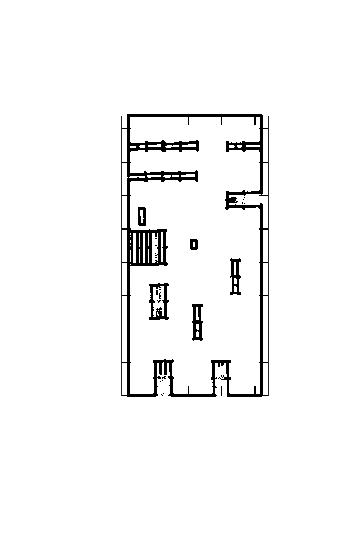
\includegraphics{./figures/09/b/map_warehouse.eps}}%
    \gplfronttext
  \end{picture}%
\endgroup

        \end{subfigure}%
        \begin{subfigure}{0.45\textwidth}\hspace{-0.2cm}
          \input{./figures/09/b/map_willowgarage.tex}
        \end{subfigure}
      \end{figure}
    \end{minipage}
  \end{overlayarea}

\end{frame}

\begin{frame}[noframenumbering]{Simulations in large environments (2/3)}

  \begin{overlayarea}{\textwidth}{\textheight}
    \leavevmode
    \begin{minipage}{0.15\textwidth}\vspace{-2cm}
      \begin{align}
        r_{\max} &= 10.0 \text{ m} \nonumber \\
        \lambda &= 360 \text{ deg} \nonumber \\
        \sigma_R &= 0.05 \text{ m} \nonumber
      \end{align}
    \end{minipage}%
      \begin{minipage}{.85\textwidth}
      \begin{figure}
        \centering
        \begin{subfigure}{0.45\textwidth}
          \centering
          \input{./figures/09/b/map_warehouse_blur.tex}
        \end{subfigure}%
        \begin{subfigure}{0.45\textwidth}\hspace{-0.2cm}
          \input{./figures/09/b/map_willowgarage_blur.tex}
        \end{subfigure}
      \end{figure}
    \end{minipage}


    \begin{textblock*}{5cm}(5.7cm,3.5cm) % {block width} (coords)
      \textcolor{black}{$\bullet$ Area $ = 745$ m$^2$ \\
                        $\bullet$ median $e_{xy} = 0.04$ m \\
                        $\bullet$ median $e_{\theta} < 1.0$ deg \\
                        $\bullet$ $94\%$ with error $< 0.5$ m \\
                        $\bullet$ median $T = 8.3$ sec}
    \end{textblock*}

    \begin{textblock*}{5cm}(11.5cm,3.5cm) % {block width} (coords)
      \textcolor{black}{$\bullet$ Area $ = 2015$ m$^2$ \\
                        $\bullet$ median $e_{xy} = 0.14$ m \\
                        $\bullet$ median $e_{\theta} = 10$ deg\\
                        $\bullet$ $90 \%$ with error $< 0.5$ m \\
                        $\bullet$ median $T = 3.7$ sec}
    \end{textblock*}

  \end{overlayarea}

\end{frame}

\begin{frame}[noframenumbering]{Simulations in 45402 environments$^*$ (3/3)}

    \begin{minipage}{0.25\textwidth}
      \begin{bw_box}
      \begin{align}
        r_{\max} = \inf \nonumber \\
        \lambda = 270 / 360 \text{ deg} \nonumber \\
        \sigma_{\bm{M}} = 0.05 \text{ m} \nonumber \\
        \sigma_R = 0.03 \text{ m} \nonumber \\
        4 \ \texttt{sm2} \text{ methods} \nonumber
      \end{align}
      \end{bw_box}
    \end{minipage}%
    \hspace{0.03cm}\begin{minipage}{.74\textwidth}
      \begin{bw_box}
        \begin{itemize}\small
          \item \textcolor{blue}{$\lambda_{\texttt{NDT}} = \lambda_{\texttt{FastGICP}} = \lambda_{\texttt{FastVGICP}} = 270$ deg} but \textcolor{magenta}{$\lambda_{\texttt{x1}} = 360$ deg}
          \item \textcolor{blue}{$\overline{e_{\mathcal{H}_1}}(\texttt{NDT}) \simeq \overline{e_{\mathcal{H}_1}}(\texttt{FastGICP}) \simeq \overline{e_{\mathcal{H}_1}}(\texttt{FastVGICP})$} \textcolor{magenta}{$\simeq \overline{e_{\mathcal{H}_1}}(\texttt{x1})$}
        \item Execution time $\sim 1.0 \text{ sec } / 100$ m$^2$ @ $1$ ray/deg
      \end{itemize}
      \end{bw_box}
    \end{minipage}

  \placebottom \vspace{-1.0cm} \tiny {* Courtesy of the Department of Computer Science, University of Freiburg, \url{http://ais.informatik.uni-freiburg.de/slamevaluation/datasets.php}}

\end{frame}


\begin{frame}[noframenumbering]{Limitations}

\begin{itemize}
\item
\begin{minipage}{.6\textwidth}
  \begin{figure}
    \input{./figures/09/a/trajectory.tex}
    \caption{\footnotesize \textcolor{exp1_blue}{Trajectory of sensor},
                           \textcolor{exp1_green}{estimated locations},\\
                           \textcolor{exp1_red}{locations with error $ > 0.5$ m}}
  \end{figure}
\end{minipage}
\item small $k$ in \texttt{bottom\_k\_poses}
\end{itemize}

\end{frame}



\input{slides/end/end.tex}


\end{document}
